\section{Introduction}
\label{sec:intro}
% Electromigration (EM) is a physical phenomenon that the metal atoms migrate along the direction of several driving forces, such as the applied electrical field. 
% With the complexity of modern very large scale integration (VLSI) designs, EM remains the top reliability failure mechanism for copper-based interconnects in all the sub-nanometer technologies.
% As a consequence of the EM effect, when the hydrostatic stress inside the metal wire reaches the critical level, resistance may varies over time during the migration, and the conducting electrons at the cathode and anode will form a void and a hillock.
% The EM crisis becomes even worse as technology advances to smaller manufacturing processes.


Electromigration (EM) is a physical phenomenon in which metal atoms migrate in response to various driving forces, such as the applied electrical field. In the context of modern very large scale integration (VLSI) designs, EM remains the dominant reliability failure mechanism for copper-based interconnects, particularly in sub-nanometer technologies. As a consequence of EM, the hydrostatic stress within the metal wire can reach critical levels, leading to resistance variations during migration. This phenomenon results in the formation of voids and hillocks at the cathode and anode, respectively, due to the accumulation and depletion of conducting electrons.
The challenges posed by EM are further exacerbated as technology advances towards nanometer manufacturing processes. In these advanced nodes, the intricate interconnect layouts and the high current densities make EM a critical concern for the long-term reliability and performance of integrated circuits. Addressing EM-related issues becomes increasingly crucial in ensuring the functional integrity and operational lifespan of semiconductor devices in modern electronics.


%The International Roadmap for Devices and Systems (IRDS) \cite{IRDS20} predicts that the allowable current density will continue to decrease due to EM, while the required current density to drive the gates will continue to increase. Developing and employing more accurate EM models and less conservative EM sign-off and assessment techniques for EM-aware designs and runtime management is critical. 

On chip power distribution network (PDN), as shown in Fig.~\ref{fig:pgimage}, is a mesh-structured network which provides power to transistors from top metals,  which has a direct impact on chip performance and reliability. Since PDNs are usually vulnerable to the EM-induced failures due to the large and unidirectional current on the PDN. In order to design robust PDN, designers have to properly size the PDN wires to meet the area and IR drop requirement. This task is changeling as the wires resistance may change over time due to the EM effect, resulting in IR drops go blow the threshold voltage  after years of aging effect.
\begin{figure}[htp]
	\centering
	\subfigure[]{
		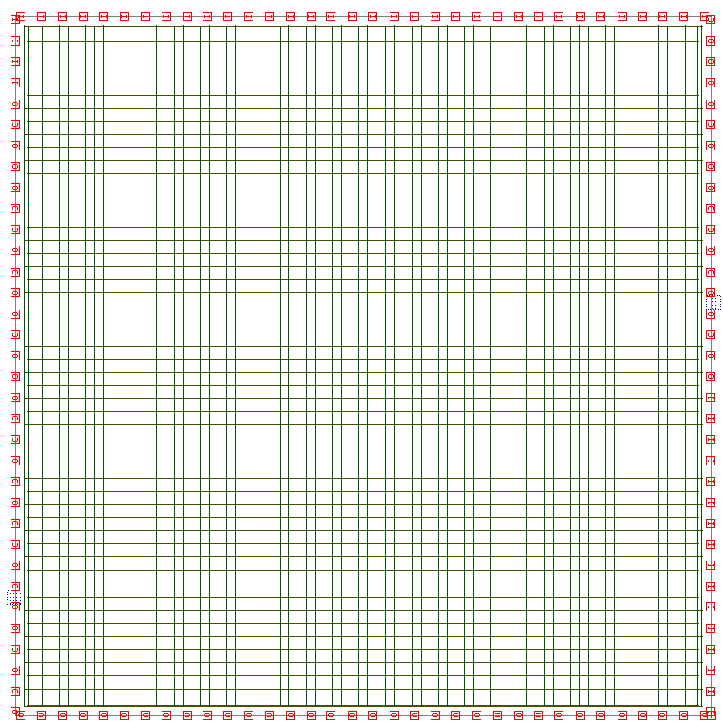
\includegraphics[width=0.4\columnwidth]{./figs/icc2pg.eps}
		\label{fig:icc2pg}}
	\subfigure[]{
		\includegraphics[width=0.48\columnwidth]{./figs/genpg.eps}
		\label{fig:genpg}}
	\caption{(a) Power and ground networks of Cortex-M0 DesignStart; (b) Voltage drop map of the power network of (a).}
	\label{fig:pgimage}
\end{figure}
% Many research works have been investigated in the past based on nonlinear or sequence of linear programming (SLP) methods~\cite{ChBr:TCAD'88,DuMa:DAC'89,Tan:DAC'99,Wang:TCAD'05,ZhouSun:TVLSI'19, Sukharev:2019pg,ZhouYu:ASPDAC'20,ZhouJin:ICCAD'20}.  Zhou {\it et al.}~\cite{ZhouSun:TVLSI'19,ZhouChen:Integration'21} proposed a power grid network sizing method based on a multi-segment EM immortality check criteria. However, the EM immortality-constrained optimization is too conservative as it requires all the interconnect trees to be immortal.  To further mitigate this issue, Moudallal {\it et al.}~\cite{Sukharev:2019pg} proposed to directly consider EM-induced IR drops instead of EM constraints on the time-varying power grid networks. It can consider post-voiding resistance change of wires based on finite difference analysis of EM-induced stress in multi-segment wires, and the resulting nonlinear problem is solved by applying successive linear programming. This method, however, still suffer high computational costs as the sensitivities of those violating nodes need to be computed by solving the circuit matrices. Recently Zhou {\it et al.}~\cite{ZhouJin:ICCAD'20, HanLiu:TCAD'22-23} proposed a conjugate gradient-based localized EM-aware IR drop fix for power grid networks, in which the gradient sensitivities were computed by the GAN (generative adversarial networks)-based deep neural network (DNN) modeling method called {\it GridNet}.

Numerous research works have investigated power grid network sizing in the past, utilizing nonlinear or sequence of linear programming (SLP) methods~\cite{ChBr:TCAD'88,DuMa:DAC'89,Tan:DAC'99,Wang:TCAD'05,ZhouSun:TVLSI'19, Sukharev:2019pg,ZhouYu:ASPDAC'20,ZhouJin:ICCAD'20}. Zhou {\it et al.}~\cite{ZhouSun:TVLSI'19,ZhouChen:Integration'21} proposed a power grid sizing approach based on multi-segment EM immortality check criteria. However, this EM immortality-constrained optimization proves too conservative, as it necessitates all interconnect trees to be immortal. In an effort to address this issue, Moudallal {\it et al.}
~\cite{Sukharev:2019pg} proposed a method that directly considers EM-induced IR drops in time-varying power grid networks. This method accounts for post-voiding resistance changes of wires through finite difference analysis of EM-induced stress in multi-segment wires, leading to a nonlinear problem solved via successive linear programming. Nonetheless, this method still incurs high computational costs, as the sensitivities of violating nodes must be computed by solving circuit matrices. More recently, Zhou {\it et al.}~\cite{ZhouJin:ICCAD'20, HanLiu:TCAD'22-23} presented a conjugate gradient-based localized EM-aware IR drop fix for power grid networks, using the GAN (generative adversarial networks)-based deep neural network (DNN) modeling method called {\it GridNet} to compute gradient sensitivities.

%The optimization is carried out based on the sensitivities method in which the sensitivities were computed by the GAN-based deep neural network (DNN) modeling method called {\it GridNet}. 

   
%GAN model is based on the standard autoencoder structures.
% and works same as a an autoencoder during the inference stage. 
Recently, variational autoencoder (VAE)~\cite{Diederik:arxiv'22} was proposed to for generative application. Compared to standard autoencoder, the encoder of VAE outputs parameters of a pre-defined distribution in the latent space for every input. Furthermore, it introduce more regulation in the cost function so that the resulting latent distribution to be close the pre-defined normal distribution, which leads to more reliable generation of new data. We notice that VAE has been used for applications such as quantum circuit for drug discovery~\cite{Li:DATE'22}, generative guided analog routing~\cite{Zhu:ICCAD'19}, and analog circuit sizing~\cite{Touloupas:SMACD'22} recently.
% gained traction as it has better interpretability of latent space, which provides them with a robust mathematical grounding and better generated result in some scenarios. Compared to the original encoder-decoder structure, VAE model improves the interpretability of latent space by encoding the input as a probabilistic distribution instead of a deterministic value.
% There are already VAE applications in the EDA field, such as Zhu {\it et al.} \cite{Zhu:ICCAD'19} adopted VAE for analog routing paradigm.
Inspired the generative capability of VAE, in this paper, we try to explore VAE for efficiently predicting the EM-aware IR drop of on-chip power grid networks to reduce the computational costs of design and optimization of  the power grid networks to ensure their IR drop and EM lifetime targets.  Our key contributions are summarized as follows:

\begin{itemlist}
% \item First, we propose a VAE-based deep neural network model, called {\it GridVAE}, to model full-chip EM-aware IR drop obtained from the numerical EM-aware IR drop analysis tool.  Compared with the latest generative adversarial network (GAN) based model~\cite{ZhouJin:ICCAD'20}, {\it GridVAE} can lead to 40$\%$ reduction in RMSE based on our synthesized power grid benchmark circuits.

\item  First, we propose a deep neural network model based on Variational Autoencoder (VAE), called {\it GridVAE}, designed to model full-chip Electromigration (EM)-aware IR drop data obtained from numerical EM-aware IR drop analysis tools. By comparing GridVAE with the latest generative adversarial network (GAN) based model~\~\cite{ZhouJin:ICCAD'20}, we observe a significant 40\% reduction in Root Mean Square Error (RMSE) based on synthesized power grid benchmark circuits.

\item Second, building upon the new VAE based EM-aware IR drop models, we leverage its differential nature to fast compute the sensitivity of cost functions with respect to the wire width. This lead to accelerated power grid wire sizing method for ensuring the EM lifetime of the chip based on sequence of linear program optimization framework. Numerical results on a number of synthesized power grid benchmarks from ARM Cortex-M0 processor designs show that the {\it GridVAE} enabled optimization can provide up to $90$X speedup over the existing analytical matrix solving-based SLP method~\cite{Sukharev:2019pg}.
 
\end{itemlist}

The rest of the paper is organized as follows: Section~\ref{sec:related} reviews the related preliminary works on the EM-induced IR drop analysis and current EM-aware power grid optimization strategy. Section~\ref{sec:strategy} introduces the VAE-based EM-aware IR drop prediction method. Experiment setup, numerical results, as long as analysis and discussions are summarized in Section~\ref{sec:results}.  Section~\ref{sec:conclusion} concludes the paper.